\documentclass[openany, a4paper, 12pt]{report}
\usepackage[utf8]{inputenc}
\usepackage{color}
\usepackage{hyperref}
\usepackage{graphicx}
\usepackage{float}

\hypersetup {
	linkcolor = {black},
	urlcolor = {blue},
	menucolor = {black},
	colorlinks = true,
}

\begin{document}

	\begin{titlepage}
		\centering
		\vfill
		{
			\bfseries
			\vskip2cm
			\Large Università di Padova\\
			\vfill
			\Huge Touhou website\\
			\Large Progetto per il corso di recnologie web\\
			\vfill
			\large Bisello Samuele, Cailotto Mirco, Todescato Matteo\\
			\vfill
			Sito web hostato all'indirizzo: www.TODO.com\\ %TODO inserire il sito
			Credenziali per l'amministrazione:\\username: admin, password: admin\\
			Indirizzo email del referente: mirco.cailotto.1@studenti.unipd.it\\
			\vfill
		}
	\end{titlepage}
	\pagenumbering{roman}
	\tableofcontents
	\newpage
	\pagenumbering{arabic}


	% Il progetto deve essere accompagnato da una relazione che ne illustri le fasi di progettazione, realizzazione e test ed evidenzi chiaramente il ruolo svolto dai singoli componenti del gruppo. Ricordo che il numero “ideale” di componenti per gruppo è di 3-4 persone. In casi particolari (da concordare col responsabile del corso, Prof. Lamberto Ballan) possono essere costituiti gruppi di 2 persone.

	% Nella relazione deve essere riportata una analisi iniziale delle caratteristiche degli utenti che il sito si propone di raggiungere. Le pagine web devono essere accessibili indipendentemente dal browser e dalle dimensioni dello schermo del dispositivo degli utenti. Considerazioni riguardanti diversi dispositivi (laddove possibile) verranno valutate positivamente.

	% La relazione deve contenere in prima pagina:
	%indirizzo web del sito;
	%eventuali password degli utenti da utilizzare in fase di correzione (una coppia login-password per ogni classe di utenza), in particolare:
	%l'utente amministratore, se presente, deve avere login e password uguali ad admin;
	%l'utente semplice, se presente, deve avere login e password uguali ad user;
	%indirizzo email del referente del gruppo per eventuali comunicazioni;
	%i file PHP devono avere i permessi corretti;
	%il sito deve utilizzare link relativi in modo da poter essere facilmente installato anche su server o cartelle diverse (se l'installazione necessita di operazioni particolari queste devono essere indicate chiaramente in relazione).

	\chapter{Abstract}
	Il progetto sviluppato propone la realizzazione di un sito web che fornisce informazioni riguardo al videogioco Touhou.\\
	Il primo obiettivo è attirare utenti che cercano delle informazioni in merito al media, probabilmente perchè lo hanno conosciuto attraverso qualche immagine satirica sui social network (come ad esempio Facebook, Reddit e 4chan) o filmati ironici su piattaforme di streaming(come ad esempio YouTube).\\
	Il secondo obiettivo è di fornire informazioni più approfondite a coloro che hanno già una conoscenza base del videogioco, fornendo notizie di attualità e consentendogli di commentare per poter creare un senso di community.\\
	Un obiettivo desiderabile è quello di raccogliere abbastanza utenza per permettere la collaborazione con manifestazioni legate ad ambiti giovani per la realizzazione di conferenze ed eventi dedicati al media.\\
	Gli obiettivi prefissati si basano sull'operato del sito web Distopia Evangelion (http://distopia.altervista.org, realizzato con Wordpress), che tratta notizie relative ad una serie animata giapponese (Neon Genesis Evangelion) e collabora con altri portali web e con organizzatori di alcune manifestazioni per la realizzazione di conferenze.\\
	Gli obiettivi precedentemente riportati sono da considerarsi puramente teorici e finalizzati alla realizzazione di un sito web con tali caratteristiche, in quanto attualmente non c'è l'intenzione di pubblicare il sito web.

	\chapter{Installazione}
	Il sito richiede un database MySql, per la creazione delle tabelle utilizzate si possono usare i due file .sql allegati, "database.sql" e "database vuoto.sql", che generano rispettivamente il database con tutti i dati inseriti nel sito web consegnato e un database con le tabelle vuote, con solo l'amministratore presente, le cui credenziali sono admin:admin.\\
	Successivamente si dovrà modificare il file dbConnection.php, presente nella root del sito, indicando i dati per l'accesso al database (HOST\_DB, USER, PASSWD, DATABASE) e la pagina di errore dove ridirigere l'utente in caso di errore nel database  (\$connectionErrorPage).\\
	La pagina di errore del database è stata lasciata configurabile in quanto nel caso di problemi al database che richiedono una lunga manutenzione, ad esempio uno spostamento del database o una dimenticanza del rinnovo dell'account del database, si può ridirigere l'utente a un secondo host temporaneo dove sono presenti i contenuti richiesti.\\

	\chapter{Progettazione}

	\section{Descrizione della sessione}
		In questa sezione del documento si andranno ad approfondire tutti gli aspetti legati alla progettazione del sito web.

	\section{Analisi della classe di utenza}

		\section{Descrizione della sessione}
		Questa sezione si pone come obiettivo l'analisi di tutte le tipologie di utenti che potrebbero navigare sul sito web, ponendo particolare attenzione alle informazioni che cercano.
		\section{Analisi dell'utenza}
		\subsection{Utente che cerca informazioni riguardanti il videogioco}
		La prima tipologia di utenti del sito sono coloro che conoscono il videogioco Touhou per fama, ma non lo hanno mai giocato. Per consentire loro di avere un'idea immediata sulla tipologia di gioco vengono presentati in home page alcuni screenshot del videogioco.\\
		Per trasmettere un'informazione più dettagliata è stata creata la pagina gameplay, che solitamente è il primo termine che viene ricercato dai videogiocatori quando desiderano comprendere le meccaniche di un determinato titolo.\\
		Usualmente questi utenti utilizzano come dispositivi pc potenti e con risoluzioni elevate, di solito uguali o superiori 1080p, ed una connessione internet veloce.
		\subsection{Utente che cerca informazioni riguardanti un singolo contenuto}
		Questa categoria di utenti è sicuramente la meno omogenea. Si tratta di utenti che vengono a conoscenza di alcune caratteristiche del videogioco attraverso immagini o filmati satirici (definiti anche "memi") presenti in rete e desiderano conoscerne la fonte.\\
		Questi utenti troveranno nella home page, appena sotto agli screenshot del gioco, alcune immagini che faranno capire subito, anche senza guardare il menu, che nel sito sono trattati anche questi aspetti.\\
		L'accesso non sarà eseguito unicamente dalla home page del sito, ma probabilmente potrebbero accedere direttamente alla pagina "Popolarità" attraverso una ricerca effettuata su motori di richerca come Google o Bing. Per tale motivo sono state inserite nella sidebar alcune notizie relative al videogioco che potrebbero attirare l'attenzione e allungare la permanenza nel sito.\\
		Questa tipologia di utenza è probabile abbia una buona conoscenza dell'inglese ed usi una vasta gamma di dispositivi recenti, come ad esempio smartphone, tablet o notebook.\\
		\subsection{Utente che cerca approfondimenti}
		Gli utenti che ricercano approfondimenti riguardo al franchise solitamente conoscono e giocano già a Touhou, quindi si presume navighino utilizzando un pc. Tuttavia Touhou è un videogioco 2D che non richiede un hardware potente e quindi non si può presumere che venga utilizzato un pc di ultima generazione.\\
		Di solito questi utenti hanno una buona conoscenza della lingua inglese e una conoscenza basilare del giapponese. Per esempio riescono a leggere i caratteri hiragana e riconoscono alcuni termini.\\
		Questi utenti cercheranno soprattutto degli approfondimenti riguardanti i molteplici personaggi oppure delle informazioni recenti riguardanti i capitoli del franchise.\\
		A questa tipologia di utenti è dedicata anche l'ultima parte della home del sito, in quanto sicuramente saranno interessati ad eventi riguardanti Touhou e quindi li si informa di questa intenzione.

	\section{Progettazione della base informativa}
		Il sito web si pone l'obiettivo di veicolare diversi contenuti, alcuni statici ed altri dinamici.
	\subsection{Contenuti statici}
		\subsubsection{Gameplay}
		Il primo contenuto sarà una panoramica del gioco, analizzando gli aspetti relativi all'usufruizione di uno dei capitoli della serie di videogioco, indicando a coloro che non lo conoscono di quale genere videoludico stiamo parlando e sottolineando le particolarità che hanno reso celebre il franchise.
		\subsubsection{Sviluppo}
		In questa pagina si parlerà dell' evoluzione di Touhou nel tempo, analizzando le "generazioni" che ha percorso dal primo videogioco, uscito nel 1996, fino all'ultimo.
		\subsubsection{Popolarità}
		Questa parte del sito tratterà i contenuti che hanno riscosso una notevole popolarità su internet e che sono legati al franchise (come ad esempio le colonne sonore, le parodie o i "meme"), cioè contenuti divertenti e molto riconoscibili, proposti e riproposti moltissime volte adattandoli ad ambiti anche molto diversificati.
		\subsubsection{Personaggi}
		La sezione relativa ai personaggi elencherà le principali entità presenti nel videogioco, fornendo per ognuna di esse le caratteristiche ed una breve descrizione.

	\subsection{Contenuti dinamici}
		\subsubsection{News}
		L'area news tratterà le ultime notizie riguardanti la serie di videogiochi, come ad esempio la pubblicazione di demo dei futuri capitoli da parte di ZUN, curiosità o articoli speciali sulla serie o anticipazioni.

		\subsubsection{Commenti degli utenti}
		Gli utenti avranno la possibilità di lasciare dei commenti sotto ogni articolo e leggere quelli altrui, in modo tale da fornire un minimo di iterazione con l'utenza.

		\subsubsection{Capitoli}
		L'ultima parte del sito elencherà i capitoli ufficiali del videogioco, correlati dall'immagine di copertina, il titolo tradotto in inglese, in italiano ed altre informazioni che possono risultare interessanti agli utenti del sito.\\
		Questa parte sarà dinamica in quanto i capitoli escono relativamente di frequente, quindi si vuole lasciare all'amministratore la possibilità di inserirne di nuovi, o di cancellare quelli che presentano informazioni errate o non aggiornate.

	\section{Strutturazione del sito}
	\subsection{Impaginazione}
	Il sito utlizza un layout a tre pannelli nella versione per dispositivi desktop.\\
	La sidebar, contenente informazioni aggiuntive, è posizionata sul lato destro in quanto offre informazioni secondarie. Perciò nella lettura europea (da sinistra a destra) sarà notata dopo il contenuto, mentre nella versione tablet o mobile sarà posizionata sotto il contenuto.\\
	Il menu del sito presenta una navigazione a schede, che nella versione per dispositivi mobili viene sostituita da un menu ad hamburger.\\
	Nel footer del sito sono presenti i crediti, la licenza dei contenuti del sito e l'accesso all'area di amministrazione.

	\chapter{Realizzazione}
	\section{Descrizione della sessione}
	In questa parte del documento si andranno ad approfondire tutti gli aspetti legati alla realizzazione del sito web.

	\section{Scelte tecniche}
	\subsection{XHTML1.1}
	Come linguaggio di marcatura si è scelto di utilizzare XHTML 1.1, tecnologia il cui uso è stato concesso dal professore Lamberto Ballan.\\
	Si è preferito l'utilizzo di XHTML 1.1 per l'aggiunta del tag ruby, il quale consente l'utilizzo del furigana (per ulteriori approfondimenti fare riferimento all'ultima sezione di questo documento relativa all'utilizzo della lingua straniera).\\
	In mancanza di supporto da parte di un browser di questa funzionalità il furigana viene semplicemente mostrato dopo la parola, in modo da non compromettere la fruizione dei contenuti.

	\subsection{JavaScript}
	Si è scelto di utilizzare JavaScript come componente marginale del sito garantendo, anche se disabilitato, che tutte le funzionalità rimangano accessibili e perfettamente funzionanti.\\
	Non sono state utilizzate librerie esterne (come ad esempio jQuery) per non appesantire il sito web, dato che il suo uso sarebbe comunque stato marginale e non avrebbe migliorato di molto la qualità della navigazione.

	\section{Suddivisione di struttura, presentazione e comportamento}
		\subsection{Parte utente}
			\subsubsection{Struttura}
			I file delle pagine della parte utente del sito sono collocate nella root del server, i file necessari alla formattazione dello stile del sito per i vari dispositivi sono collocati nella cartella style mentre le immagini necessarie al sito sono collocate nella cartella images, la quale presenta la suddivisione per le immagini delle news, i personaggi e per i capitoli. I file contenenti gli script necessari al sito sono collocati nella cartella script.
			\subsubsection{Presentazione}
			La presentazione della pagina è realizzata tramite file css, il principale sono style, che viene utilizzata per ogni pagina.\\
			In caso di dispositivo mobile o tablet vengono utilizzati due stili extra, tablet e mobile, che hanno il compito di far cambiare la presentazione della pagina per meglio adattarla a schermi di dimensioni inferiori.\\
			Per quanto riguarda la stampa è stato creato un foglio stile, chiamato print, che rimuove tutti i contenuti non necessari e impagina le informazioni per meglio adattarle a un foglio A4.\\
			Si è scelto di rimuovere il menu, ma di lasciare il titolo e la breadcrumb, in modo tale da aiutare l'utente a ritrovare il sito web e la pagina nel caso non si ricordasse la fonte.\\
			Le immagini sono state rimosse, ad eccezione delle immagini dei personaggi, che sono stati valutate come molto utili per una veloce consultazione.

			\subsubsection{Comportamento}
			Il comportamento della pagina è stato gestito tramite JavaScript per il controllo delle form, per i commenti e per fornire la possibilità di ingrandire le immagini all'interno della pagina. Sono presenti anche controlli tramite codice PHP per garantire che il sito continui a funzionare corretamente anche in caso di assenza dell'interprete JavaScript.
			
			\begin{figure}[H]
				\centering
				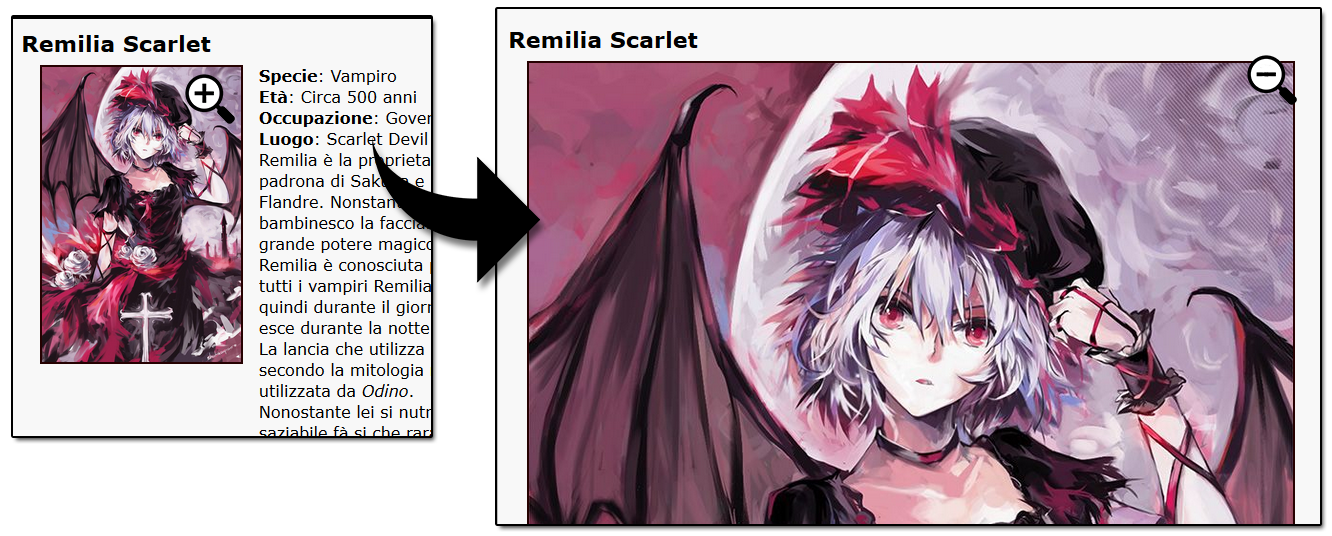
\includegraphics[width=0.8\linewidth]{images/zomm}
				\caption{Funzione di zoom implementata in JavaScript}
			\end{figure}
			
			Tutto il codice PHP relativo all'esecuzioni di azioni, come l'aggiunta dei commenti, è stato completamente diviso da quello utilizzato per la visualizzazione dei contenuti.\\

	\subsection{Parte amministratore}
		\subsubsection{Struttura}
		generazione di visualizzazione dei dati nel db
		\subsubsection{Presentazione}
		Lo stile delle pagine per l'amministrazione differisce rispetto alla parte utente, in quanto dal lato amministratore sono stati rimossi alcuni elementi inutili, come il footer e la sidebar, in modo da renderla più veloce e fare spazio alle utilità necessarie all'amministrazione del sito.
		\subsubsection{Comportamento}
		La parte admin si caratterizza per un minor utilizzo dei controlli da parte di JavaScript e PHP sui form, in quanto l'amministratore ha la possibilità di inserire tag html o se lo desidera di lasciare dei campi vuoti.\\
		Questo per fare fronte ad una mancanza di un editor di test integrato che consenta una scrittura semplificata dei file HTML, in quanto svilupparlo sarebbe stato troppo oneroso per il progetto.\\
		Sono inoltre presenti tutti i controlli relativi all'SQLInjection per evitare che l'amministratore inconsapevolmente generi errori all'interno del database.\\
		Tutto il codice PHP relativo all'esecuzione di azioni è stato completamente diviso da quello utilizzato per la visualizzazione dei contenuti, ad eccezione dell'index della pagina di amministrazione.\\
		La pagina che richiede il login della parte di amministrazione e la visualizzazione della pagina introduttiva è la medesima. Si è scelta questa soluzione per consentire il salvataggio di un segnalibro da parte degli amministratori, i quali verranno portati alla pagina di login qualora non siano stati autenticati. In caso contrario, verranno direttamente trasferiti alla pagina principale di amministrazione, senza ulteriori redirect.

	\chapter{Validazione e test}
		\section{Descrizione della sessione}
			Questa sezione si occupa di metodo e strumenti con i quali si sono svolti i processi di verica e validazione delle componenti del sito.
		\section{Validazione con test automatici}
			\subsection{Markup Validation Service w3.org}
				Tutte le pagine sono state testate con il validatore fornito da w3.org, la verifica non ha segnalato nessun problema in nessuna pagina, con l'eccezione di un warning "Using Direct Input mode: UTF-8 character encoding assumed" a causa dell'utilizzo della modalità di input diretto del codice HTML.\\
				Sono state testate anche la pagina di login, la pagina di database non raggiungibile e la pagina di errore di input, tutte con esito positivo.
			\subsection{W3C CSS Validator w3.org}
				Tutti gli stili css sono stati testati con il validatore fornito da w3.org, compreso quelli di stampa, e non sono stati rilevati errori.
				%TODO - Samu e i Warning per Apple
				
			\subsection{Vamola validator}
				Uno strumento utilizzato per la verifica automatica dell'accessibilità è stato Vamola, presente all'indirizzo \url{www.validatore.it/vamola_validator/checker/index.php}.\\
				Come impostazione è stato utilizzato "WCAG 2.0 (Level AAA)", tutti i potenziali problemi che vengono segnalati raccolgono tutti elementi che il validatore non sa come controllare e quindi viene richiesta una supervisione umana, come ad esempio ogni alt.\\
				Nessun errore è stato segnalato.
			\subsection{WAVE Accessibility Extension}
				Un altro strumento utilizzato per la verifica dell'accessibilità è stato WAVE, disponibile per il browser Firefox all'indirizzo \url{https://addons.mozilla.org/it/firefox/addon/wave-accessibility-tool/}, del quale esiste anche una versione per Google Chrome sul relativo store.\\
				Il plugin ha segnalato alcuni warning riguardanti gli alt, che richiedevano un controllo manuale, e alcuni warning relativi ai furigana rappresentati con una font non molto grande, ma che secondo una nostra analisi manuale è ritenuto sufficientemente grande in quanto supplementare alla lettura.\\
				Un errore segnalato riguarda una label mancante per un input nella pagina di aggiunta delle news, ma in quel caso l'input è nascosto dall'utente essendo l'indicazione di quale articolo si sta modificando, quindi anche nel caso di uno screen reader non verrebbe visualizzato, per queste motivazioni una label risulterebbe inappropriata.
			\subsection{Web Accessibility Toolbar (WAT)}
				Il sito è stato testato su Internet Explorer 11 utilizzato WAT.\\
				Purtroppo il plugin non è aggiornato e presenta molti strumenti inutilizzabili, la versione corrente è stata scaricata da:\\ \url{https://github.com/ThePacielloGroup/WebAccessibilityToolbar}.\\
				Uno strumento funzionante molto utile è Juicy Studio Luminosity Analyzer, che ha analizzato il contrasto dei colori, fornendo come indice minimo 7.07, sufficiente per avere la certificazione WCAG 2.0 AAA.\\

			\subsection{Total Validator}
			Per permettere la verifica delle pagine di amministrazione a Total Validator Basic è stata temporaneamente rimossa la verifica del login, questo ha portato ad alcuni errori nella pagina di gestione degli account, in quanto l'account correttamente in uso era invalido.\\
			Un warning sollevato in ogni pagina è riguardante il link interno per saltare al contenuto, precisamente "W874 Add a skip navigation link as the first link on the page", che viene sollevato in quanto il testo non è "Skip to main content", bensì "Vai al contenuto", in quanto il sito è mirato ad utenti italiani.\\
			Da precisare che oltre alla presenza del link per andare al contenuto è disponibile anche un link per tornare ad inizio pagina, inserito per facilitare la navigazione da dispositivi tascabili.\\
			Altri warning presenti sono in riferimento ad immagini che presentano alt vuoti, in tutti i casi segnalati si tratta di immagini puramente decorative oppure che non veicolano una informazione che può essere descritta. Un esempio sono le copertine dei capitoli del videogioco, che presentano motivi e colori imprecisati oppure illustrazioni senza un  significato, utilizzate come riempitivo per la copertina.

			\subsection{Vischeck}
			\`{E} stato utilizzato il sito web \url{vischeck.com} per controllare i colori in caso di daltonismo, che non ha evidenziato particolari problemi alla individuazione della suddivisione del sito o dei contenuti.
			
			\begin{figure}[H]
				\centering
				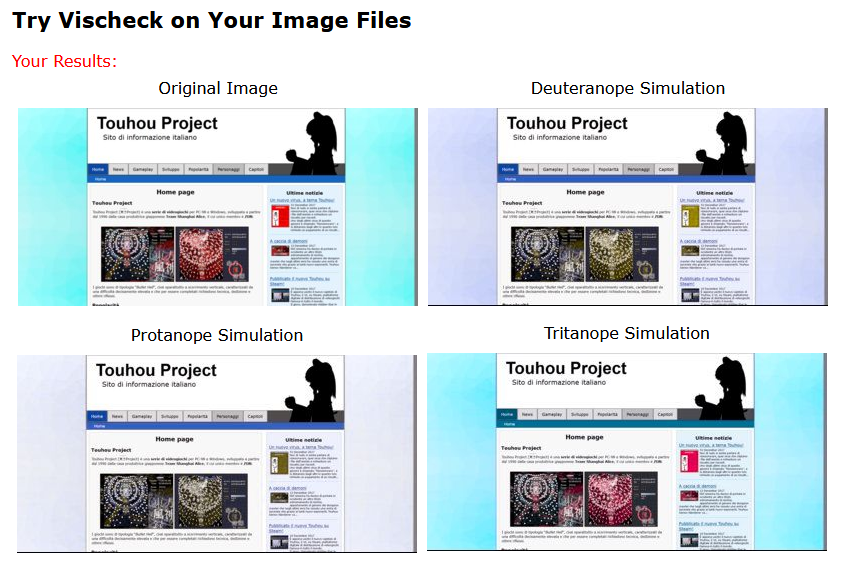
\includegraphics[width=0.8\linewidth]{images/daltonismo}
				\caption{Risultati ottenuti su Vischeck}
			\end{figure}
			Ulteriormente anche su mobile sono state testata le stesse varianti di colorazione agendo sulle impostazioni di sviluppo di Android 7.1 presenti sulla rom MIUI versione China Dev, purtroppo gli screenshots effettuati in questa modalità di colore apparivano senza filtro, e per questo motivo non è stato possibile riportare i test effettuati in questo documento.

		\section{Test su diversi dispositivi}
			Il sito è stato testato su varie macchine e sistemi operativi. Nelle sezioni seguenti verranno elencati assieme ai browser e alle risoluzioni testate.
				\subsection{Windows 10}
				Sono state testate le risoluzioni di 1080p e 2160p con i browsers:
				\begin{itemize}
					\item Firefox Quantum
					\item Google Chrome
					\item Firefox 56
					\item Waterfox 57
					\item Edge
					\item Chromium 64
					\item Mozilla Firefox 3
					\item Internet Explorer 11
				\end{itemize}
				Mozilla Firefox 3 utilizza una dimensione errata dell'immagine nella testata. Questo aspetti rovinano leggermente il rendimento grafico ma non compromettono le funzionalità, in quanto tutti i contenuti risultano perfettamente fruibili dall'utente.\\
				Un Secondo appunto riguardante Firefox 3 è l'incompatibilità con parte del codice JavaScript: solamente il controllo della compilazione dei campi di testo funziona correttamente.\\
				Internet Explorer 11, con la modalità Explorer 7, non genera nessun problema, ed anche il problema della dimensione della testata riscontrato su Firefox 3  è assente; anche con Microsoft Edge 16 (ultima versione) non sono stati riscontrati problemi. \\
				Non sono stati rilevati ulteriori problemi o incompatibilità con i browser sopra menzionati, anche variando la grandezza del font, dello zoom della pagina, della dimensione della finestra e disattivando JavaScript.
%TODO: come si comporta su EDGE? io non lo ho

				\subsection{GNU/Linux Fedora 27}
				Sono state testate le risoluzioni di 1800p e 2160p con i browsers:
				\begin{itemize}
					\item Firefox Quantum
					\item Google Chrome
					\item Firefox 56
					\item Lynx
				\end{itemize}
				Durante la fase di test su questa piattaforma non sono emerse problematiche a livello di compatibilità o visibilità nonstante le alte risoluzioni. In oltre su questa piattaforma è sata testa la leggibilità del sito con l'utilizzo del browser cli Lynx.

				\subsection{MacOS High Sierra}
				Sono state testate le risoluzioni di 1800p, 2160p e 2880x1800p con i browsers:
				\begin{itemize}
					\item Safari
					\item Firefox Quantum
					\item Google Chrome
					\item Firefox 56
				\end{itemize}

				\subsection{FreeBSD 11}
				\`{E} stata testata con il browser Lynx utilizzando la console senza x11, quindi da terminale, e con x11, quindi da una finestra di emulazione del terminale di dimensione variabile.

				\subsection{Dispositivi mobili}
				Di seguito sono elencati i vari dispositivi mobili sui quali il sito è stato testato
				\begin{itemize}
				\item Testato su Xiaomi Redmi 4x con Miui browser, Firefox Rocket e Waterfox con una risoluzione di 720p
				\item Kindle touch 7' generazione con schermo e-ink in bianco e nero, con una risoluzione di 800x600 e con il browser sperimentale fornito di default.
        		\item Testato su Ipad Pro 10.5' su browser Safari (devo aggiungere la versione), con una risoluzione di 2224x1668
				\end{itemize}
		\section{Test con diverse impostazioni utente}
			\subsection{Nome Sottosezione}
		\section{Lynx e come potrebbe essere se letto}
			\subsection{Nome Sottosezione}

	\chapter{Ambiguità incontrate e scelte intraprese}
		\section{Descrizione della sessione}
			In questa sezione del documento sono elencate tutte le decisioni prese su aspetti ambigui presenti nel sito\\
		\section{Utilizzo della lingua straniera}
			\subsection{Furigana}
				A supporto dei termini scritti in kanji, sono stati inseriti i furigana, cioè la pronuncia del termine in caratteri hiragana (pratica comune in siti che presentano termini giapponesi mirati ad adolescenti o a stranieri che potrebbero avere una discreta conoscenza del giapponese).\\
				Questo avviene anche in Giappone in quanto i kanji essendo molteplici (si calcola circa 18'000) è frequente che i lettori ne trovino di sconosciuti e si cerca di aiutarli inserendo a lato la pronuncia nel sillabario utilizzato per i termini giapponesi, cioè l'hiragana.\\
				A volte, se il termine è di origine straniera, il furigana potrebbe presentarsi con caratteri del sillabario katanaka. Questo avviene di rado e non è presente nel nostro sito, in quanto preferiamo presentare le parole inglesi direttamente in alfabeto latino.
			\subsection{Traslitterazioni}
				Le traslitterazioni dalla lingua giapponese sono spesso imprecise e ci sono controversie sulla pronuncia persino nella stessa lingua giapponese; quindi si è scelto, in caso di screen reader, di lasciare leggere le parole traslitterate usando l'alfabeto italiano, che si rivela anche più preciso rispetto all'inglese nella lettura dei termini.\\
				Alcune parole giapponesi, che si rivelano essere lette più fedelmente dalla pronuncia inglese, sono state marcate come tali.\\
				Se le parole traslitterate fossero state marcate come lingua giapponese i termini sarebbero stati considerati in alfabeto "romaji" (romano, cioè l'alfabeto latino), e quindi traslitterati nuovamente in katakana per poi essere letti usando la lingua giapponese, che avrebbe portato a pronunce errate, in quanto non c'è una corrispondenza precisa tra l'alfabeto e il sillabario.
			\subsection{Termini errati}
				Nel sito appaiono termini con delle lettere maiuscole poste senza rispettare la grammatica inglese. In quei casi si è trascritto il termine esattamente come appare nella documentazione ufficiale, all'interno del videogioco o nei file dello stesso. Alcuni esempi sono "Nights of Night" o "U.N. Owen Was Her". In questo ultimo caso non ci è dato sapere cosa significhi U.N., si pensa possa essere un riferimento a Una Nancy Owen, ma non essendoci alcuna conferma ufficiale è stato preferito ometterlo.\\

	\chapter{Suddivisione del lavoro}
	\section{Descrizione della sessione}
	\section{Suddivisione per membro del gruppo}
	\subsection{Bisello Samuele}
	\begin{itemize}
		\item Scrittura contenuti per la pagina capitoli
		\item	Stile login
		\item Controllo form lato admin
		\item	Parte dello sticky header
		\item Test su  MacOS High Sierra (v10.13.2)
		\item
		\item
	\end{itemize}
	\subsection{Cailotto Mirco}
	\begin{itemize}
		\item Creazione struttura base del sito
		\item Scrittura contenuti per pagina di home page, gameplay, realizzazione, popolarità
		\item Creazione php per le pagine dinamiche, compresa la parte di amministrazione
		\item Creazione stile per le pagine home page, news, articoli, gameplay, realizzazione, popolarità e capitoli
		\item Scrittura della funzione php per l'upload delle immagini
		\item Scrittura del sistema di errori forniti all'utente
		\item Parsing degli input per evitare SQLInjection
		\item Creazione sistema di caching per la sidebar
		\item Creazione della struttura del database
		\item Controllo dei valori inseriti dagli utenti generici
		\item Stesura dello scheletro della relazione
		\item Stesura parte abstract, di analisi dell'utenza e di ambiguità linguistica della relazione
		\item
	\end{itemize}
	\subsection{Todescato Matteo}
	\begin{itemize}
		\item Scrittura contenuti per pagina dei personaggi
		\item Gestione degli amministratori nella parte php e relativa tabella
		\item Controllo per il login
		\item Script per la validazione delle form lato utente
		\item Inserimento notizie
		\item Test su sistema Linux
		\item
		\item
		\item
	\end{itemize}

\end{document}
